\chapter{بسته نرم‌افزاری تهیه شده برای کار با مدل‌های آمیخته} \label{ch:mixest}
%TODO tell about why using max lik framework
در فصل
\ref{ch:mixtureModels}
به تعدادی از مشکلات موجود هنگام تخمین پارامترهای مدل‌های آمیخته در چارچوب درست‌نمایی بیشینه اشاره نمودیم.
مهم‌ترین این مشکلات، موارد زیر هستند:

\begin{itemize}
\item 
بی‌کران شدن درست‌نمایی: به عنوان مثال هنگامی که یکی از اجزا تعداد کمی از نقاط نزدیک به هم را در بر می‌گیرد درست‌نمایی به سمت بی‌نهایت میل می‌کند%
~\cite{ciuperca_penalized_2003}.

\item
بیشینه‌های محلی: با توجه به این که تابع لگاریتم درست‌نمایی استفاده شده در تخمین پارامترهای مدل‌های آمیخته به طور معمول دارای نقاط کمینه و بیشینه محلی زیادی است، یافتن نقطه بهینه پیچیده خواهد بود%
~\cite{ueda_split_2000}.

\item
تعداد درست اجزای مدل: در بسیاری از کاربردها می‌بایست تعداد مناسب اجزای مدل آمیخته نیز در کنار پارامترهای آنها تخمین زده شود و این تعداد از قبل مشخص نیست%
~\cite{khalili_variable_2007}.
\end{itemize}

متاسفانه کتابخانه‌های نرم‌افزاری موجود برای کار با مدل‌های آمیخته، امکان رسیدگی به این مشکلات را هنگام استفاده از مدل‌های مخلوط در چارچوب درست‌نمایی بیشینه برای حل مسائل مختلف و به خصوص مسائل با ابعاد بالا و دادگان بزرگ، فراهم نمی‌کنند و پیاده‌سازی راه‌حل‌های مناسب جهت رسیدگی به این مسائل، می‌تواند وقت و انرژی زیادی را از پژوهشگران بگیرد.
لذا با توجه به گستردگی کاربردهای مدل‌های آمیخته در علوم مختلف، بر آن شدیم تا یک کتابخانه نرم‌افزاری منسجم جهت کار با مدل‌های آمیخته به صورت یک
{\mmm{جعبه ابزار}{toolbox}}
در محیط نرم‌افزار \lr{MATLAB} تهیه نماییم که علاوه بر استفاده در پروژه حاضر، امکان استفاده از آن برای عموم پژوهشگران میسر باشد.
جعبه ابزار تهیه شده با عنوان
\lr{MixEst}
و به صورت
{\mmm{متن باز}{open source}}
از طریق آدرس اینترنتی
\lr{\textit{visionlab.ut.ac.ir/mixest}}
در دسترس عموم قرار دارد%
~\cite{hosseini_mixest_toappear}.

\section{معرفی}
جعبه ابزار
MixEst
یک بسته نرم‌افزاری قدرتمند و با کاربری آسان است که بسیاری از راهکارهای جدید ارائه شده جهت رسیدگی به مسائلی که درمورد مدل‌های آمیخته مطرح گردید در آن پیاده‌سازی شده است.
کاربران می‌توانند از این جعبه ابزار به عنوان یک میز آزمایش برای مدل‌های آمیخته استفاده کنند که یک
{\mmm{واسط برنامه‌نویسی نرم‌افزار}{Application Programming Interface (API)}}
ساده و منسجم همراه با انتخاب‌های فراوان جهت انجام انواع پژوهش‌ها با استفاده از این مدل‌ها را برایشان فراهم می‌کند.
در عین حال در پیاده‌سازی الگوریتم‌ها و محاسبات، داشتن کارآیی بالا خصوصا هنگام کار با دادگان بزرگ مورد توجه قرار گرفته و کاربران می‌توانند از این بسته در کاربردهای عملی نیز استفاده نمایند.
فراخوانی این توابع به سادگی به شکل زیر انجام می‌شود:
\begin{latin}
\begin{lstlisting}
data = D.sample(theta, 1000);
\end{lstlisting}
\end{latin}
توضیحات کامل مربوط به توابع مختلف ارائه شده توسط توزیع‌ها در مستندات مربوط به توابع در بسته نرم‌افزاری آمده است.
در این‌جا به طور مختصر، اصول ابتدایی کار با این توابع را بیان می‌نماییم.
دستور بالا، تابع
\mcode{sample}
را از توزیع
\mcode{D}
فراخوانی می‌کند تا تعداد 1000 نمونه تصادفی را از آن توزیع استخراج نماید.
آرگومان
\mcode{theta}
پارامترهای مورد نظر برای توزیع را در بر دارد.
این آرگومان، یک ساختار ساده است که هر فیلد آن متناظر با یکی از پارامترهای توزیع می‌باشد.
به عنوان مثال اگر توزیع مربوطه همان توزیع گوسی دومتغیره که در بالا ساخته شد باشد، می‌توانیم
\mcode{theta}
را به صورت زیر بسازیم:
\begin{latin}
	\begin{lstlisting}
theta.mu = [1; 2];
theta.sigma = [2 1; 3 4];
	\end{lstlisting}
\end{latin}
به این ترتیب یک ساختار پارامتر برای توزیع گوسی دومتغیره با میانگین
(\mcode{mu})
و ماتریس کوواریانس
(\mcode{sigma})
داده شده خواهیم داشت.
همچنین می‌توان ساختارهای پارامتر را از خروجی برخی از توابع ارائه شده توسط توزیع بدست آورد.
به عنوان مثال با فراخوانی تابع
\mcode{randparam}
می‌توانیم یک ساختار پارامتر با مقادیر تصادفی برای کلیه پارامترهای توزیع بسازیم:
\begin{latin}
	\begin{lstlisting}
theta = D.randparam();
	\end{lstlisting}
\end{latin}
همچنین توابع برازش توزیع بر داده‌های مشاهده شده نیز پارامترهای تخمین زده شده را در قالب همین ساختارها بازمی‌گردانند.
نام پارامترهای استفاده شده برای هر توزیع، در مستندات تابع سازنده آن آمده است.

امکانات معمول ارائه شده از طریق ساختارهای توزیع، شامل توابعی برای محاسبه لگاریتم درست‌نمایی و گرادیان آن نسبت به پارامترها یا داده‌ها، توابع مخصوص توزیع به منظور تنظیم بهینه‌سازی و جلوگیری از بیش‌برازش، توابعی برای محاسبه تابع چگالی احتمال، تابع توزیع تجمعی، آنتروپی، توابع معیار اطلاعاتی و ... هستند که در مستندات بسته، توضیحات کاملی در مورد آن‌ها آمده است.

جعبه ابزار
MixEst
شامل پیاده‌سازی تعدادی از توزیع‌های پرکاربرد می‌باشد که در جدول
\ref{table:distributions}
فهرستی از آن‌ها را آورده‌ایم.
\begin{table}[ht]
\caption{توزیع‌های احتمال پیاده‌سازی شده در جعبه ابزار}
\label{table:distributions}
\begin{center}
\begin{small}
\begin{tabular}{cc}
\hline
\textbf{توزیع}
&
\textbf{تابع سازنده}
 \\ \hline
توزیع گوسی (نرمال چندمتغیره) &
\lr{mvnfactory} \\
توزیع آمیخته &
\lr{mixturefactory} \\
توزیع گاما &
\lr{gammafactory} \\
توزیع ECD
\lr{(Elliptically-Contoured Distribution)}
&
\lr{ecdfactory} \\
توزیع vMF
\lr{(von Mises-Fisher)}
&
\lr{vmffactory} \\
توزیع
\lr{Angular Gaussian}
&
\lr{agfactory} \\
توزیع
\lr{Multinomial Logistic} \lr{(MaxEnt Classifier)}
&
\lr{mnlfactory} \\
توزیع فاکتوریل
\lr{(Factorial)}
&
\lr{factorialfactory} \\
توزیع گوسی با تغییر پارامتر
(\cite{hosseini_manifold_2015})
&
\lr{mvn2factory} \\
توزیع آمیخته شرطی
\lr{(Mixture of Experts)}
&
\lr{moefactory} \\
توزیع گوسی شرطی
&
\lr{cmvnfactory} \\
توزیع گوسی شرطی با تغییر پارامتر
(\cite{hosseini_manifold_2015})
&
\lr{cmvn2factory} \\
گیت softmax
&
\lr{softmaxfactory} \\
\hline
\end{tabular}
\end{small}
\end{center}
\end{table}

%%%%%%%%%%%%%%%%%%%%%%%%%%%%%%%
\section{توابع تخمین پارامترها}
\label{sec:estimation_functions}
%%%%%%%%%%%%%%%%%%%%%%%%%%%%%%%
توابع تخمین در جعبه ابزار
MixEst
الگوریتم‌هایی را پیاده‌سازی می‌کنند که پارامترهای بهینه توزیع‌ها را جهت برازش به داده‌های مشاهده شده می‌یابند.
در این بخش به طور مختصر به نحوه کار با این توابع اشاره می‌کنیم.
اطلاعات دقیق‌تر در مورد هر یک از توابع در مستندات جعبه ابزار موجود است.

تابع اصلی برای برازش توزیع‌ها به داده‌ها تابع
\mcode{estimate}
است که در حالت ساده به صورت زیر قابل فراخوانی می‌باشد:
\begin{latin}
	\begin{lstlisting}
theta = D.estimate(data, options);
	\end{lstlisting}
\end{latin}
آرگومان اول ورودی این تابع،
(\mcode{data})\begin{figure}[b!]
	\begin{center}
		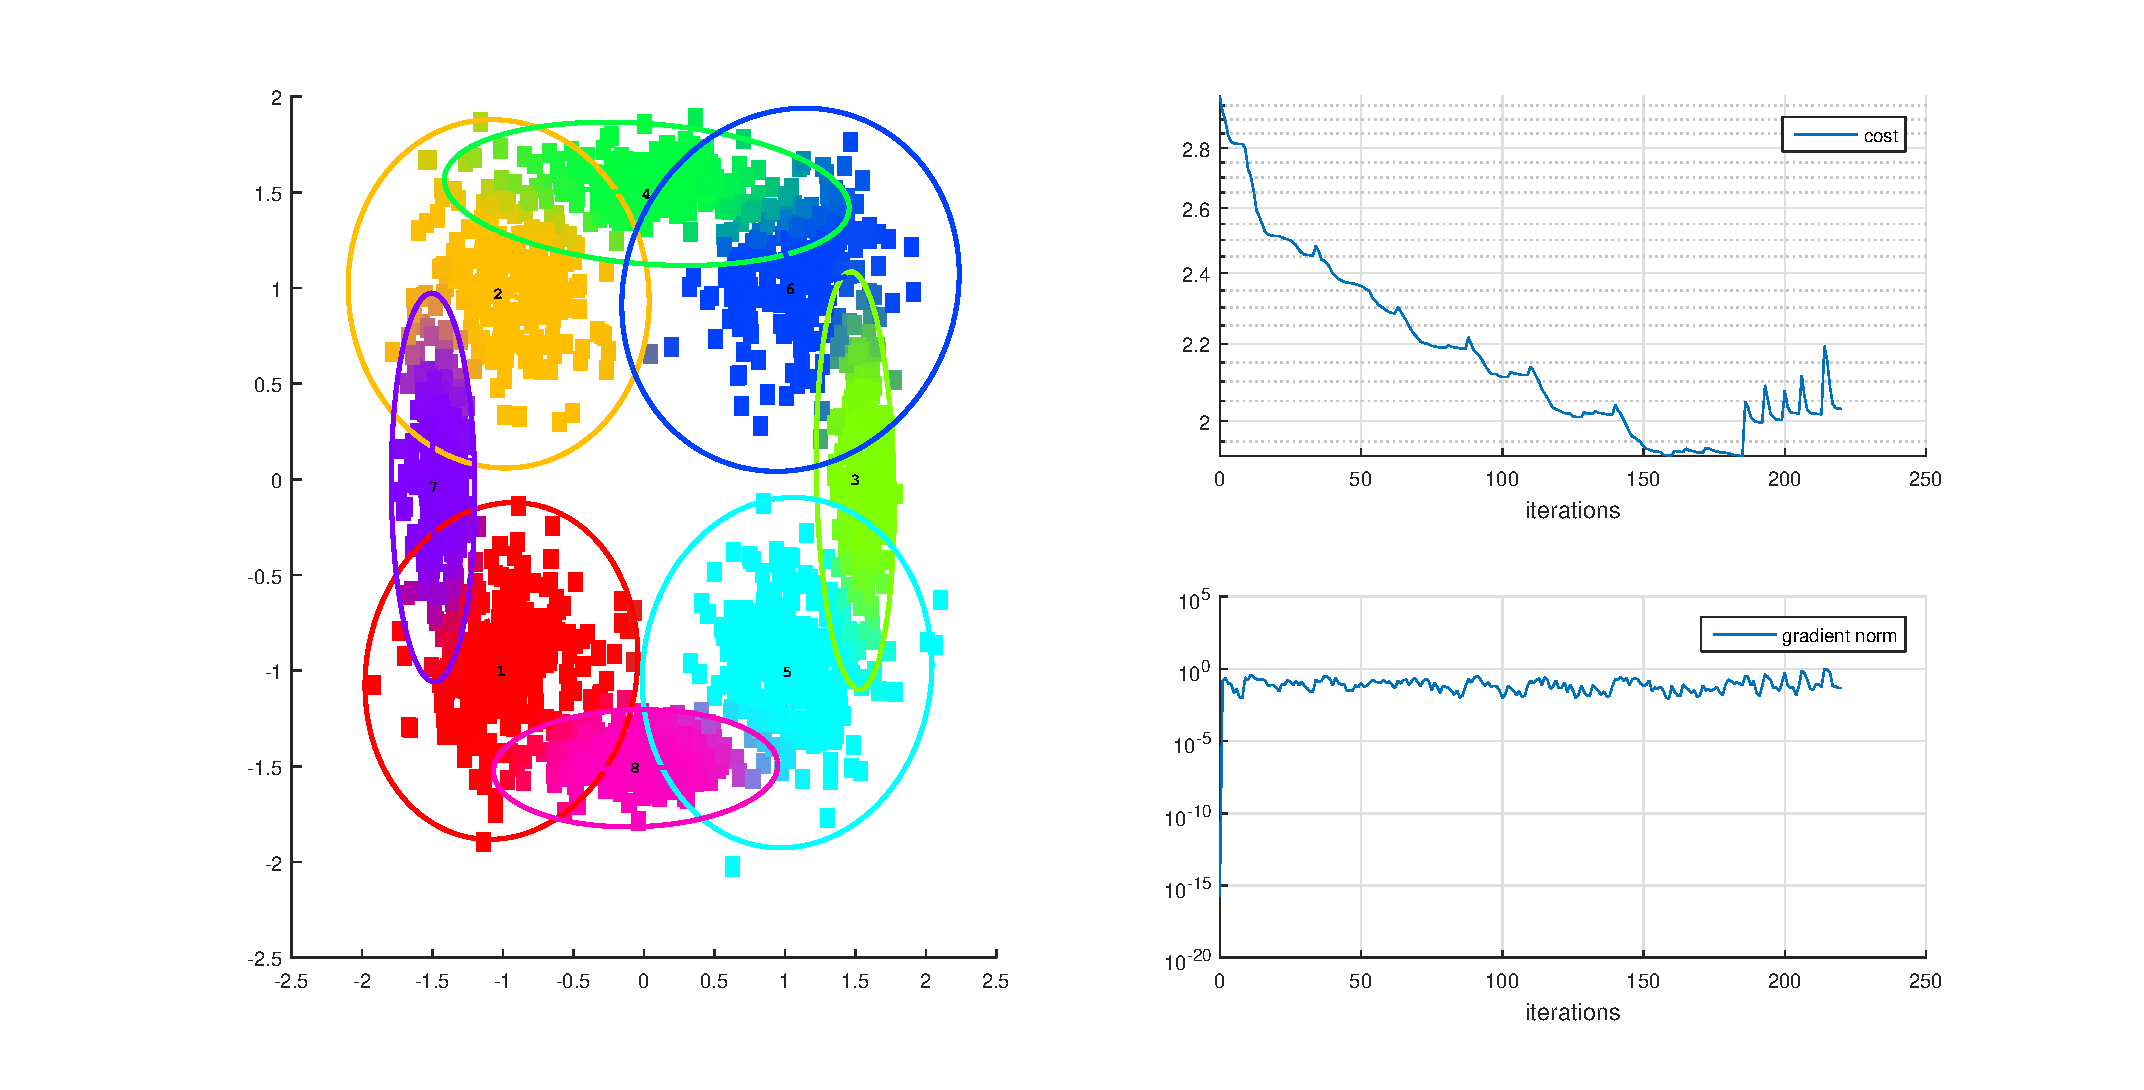
\includegraphics[width=\textwidth]{code-sample2.eps}
	\end{center}
	\caption[نمودارهای خروجی نمونه کد دوم]
	{
نمودارهای خروجی نمونه کد دوم -
نمودار سمت چپ نمایشی بصری از اجزای برازش شده مدل آمیخته گوسی را نشان می‌دهد.
در نمودارهای سمت راست، مقدار تابع هزینه و اندازه گرادیان آن در طی فرآیند تخمین رسم شده است.
		\label{fig.code-sample2}
	}
\end{figure}


\begin{latin}
\begin{lstlisting}[frame=single,numbers=left,aboveskip={\baselineskip},belowskip={1.5\baselineskip}]
load data_sm
% visualization and plotting options
figure('Units', 'normalized', 'OuterPosition', [0 0 1 1])
options.visualization.axes = subplot(2,2,[1 3]);
options.plotCost.axes = subplot(2,2,2);
options.plotCost.iterCount = Inf;
options.plotGradNorm.axes = subplot(2,2,4);
options.plotGradNorm.iterCount = Inf;
options.visualization.mixture.colorize = true;
options.visualization.stopOnClose = true;
% common estimation options
options.verbosity = 1;
options.solver = 'lbfgs';
options.tolCostDiff = 1e-3;
% split-and-merge options
options.sm.splitCriterion = 'kl';
options.sm.mergeCriterion = 'kl';
options.sm.splitInit = 'default';
options.sm.mergeInit = 'default';
options.sm.numInit = 1;
options.sm.numMin = 1;
options.sm.numMax = 15;
options.sm.mergeMaxCands = 5;
options.sm.splitMaxCands = 5;
options.sm.maxFail = 2;
options.sm.ComponentD = mvnfactory2(2);
% run
cem(data, options)
\end{lstlisting}
\end{latin}

\pagebreak %TODO?
در نمونه کد زیر، با استفاده از یک توزیع آمیخته شرطی از توزیع‌های \lr{multinomial logistic}، مجموعه داده \lr{Fisher's Iris} را طبقه بندی می‌نماییم.

\begin{latin}
\begin{lstlisting}[frame=single,numbers=left,aboveskip={\baselineskip},belowskip={1.5\baselineskip}]
% load the iris data and randomly permute them
load data_iris
index = randperm(150);
data = data(:, index);
% Use 120 points for training and 30 for test
data_train = data(:, 1:120);
data_test = data(:, 121:150);
% create a mixture of multivariate logit
datadim = 4; % data dimensions
num = 3; % number of labels
E = mnlfactory(datadim, num); % expert
G = softmaxfactory(num, datadim); % gate
D = moefactory(G, E);
% plotting options
options.plotcost = true;
% main options
options.verbosity = 2;
options.solver = 'lbfgs';
options.tolcostdiff = 1e-6;
options.crossval = true;
options.minibatch.size = 10;
options.maxiter = 200;
options.minibatch.discardhistory = false;
options.crossval.toliter = 100;
% perform estimation
theta = D.estimate(data_train, options);
% perform prediction
data_pred = D.predict(theta, data_test);
label = data_test(end,:)
data_pred
disp(['percentage of correct classification : ' num2str(sum((label-data_pred)==0) * 100 /30)]);
\end{lstlisting}
\end{latin}




